\chapter*{\hfill{}УСЛОВИЕ\hfill{}}

Для сложной системы $S$, имеющей не более 10 состояний, необходимо определить среднее время нахождения системы в предельных состояниях, то есть при установившемся режиме работы.

На вход подается матрица, на пересечении строк и столбцов которой находятся интенсивности переходов.

\chapter{Теоретическая часть}%

Случайный процесс называется Марковским, если он обладает следующим свойством: для каждого момента времени $t_0$ вероятность любого состояния системы в будущем $t > t_0$ зависит только от ее состояния в настоящем, то есть при $t = t_0$, и не зависит от того когда и каким образом система пришла в это состояние. Не зависит от того, как процесс развивался в прошлом. Для Марковских процессов хорошо работают Уравнения Колмагорова.

По модели из условия строятся уравнения Колмогорова: в левой части уравнений находится производная вероятности состояний, а правая часть содержит члены по количеству переходов, связанных с текущим состоянием. Если направление перехода в текущее состояние, то соответствующий член имеет знак минус, если направление из состояния, то плюс. Каждый член равен произведению плотности вероятности перехода на вероятость того состояния, из которого идет этот переход.

Поскольку модель имеет установившийся режим, то левые части уравненя будут равно нулю. Далее вводится уравнение нормировки и производится подсчет.

Получившиеся вероятности являются средним относительным временем пребывания системы в данном состоянии.

Среднее время находится по формуле \ref{eq:time}

\begin{equation}\label{eq:time}
    t_i = \frac{1 - p_i}{p_i \cdot \sum_{i \ne j}\lambda_{ij}}
\end{equation}

\chapter{Примеры работы}

На рисунках из данного раздела приведены примеры работы реализованной программы.

\begin{figure}[H]
    \centering
    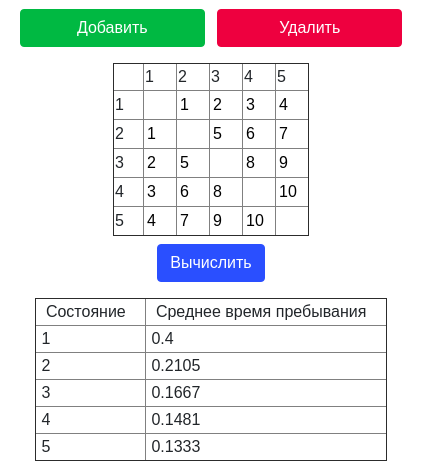
\includegraphics[width=0.6\textwidth]{images/scr01.png}
    \caption{Результат работы для системы из 5 состояний}
    \label{fig:1}
\end{figure}
\begin{figure}[H]
    \centering
    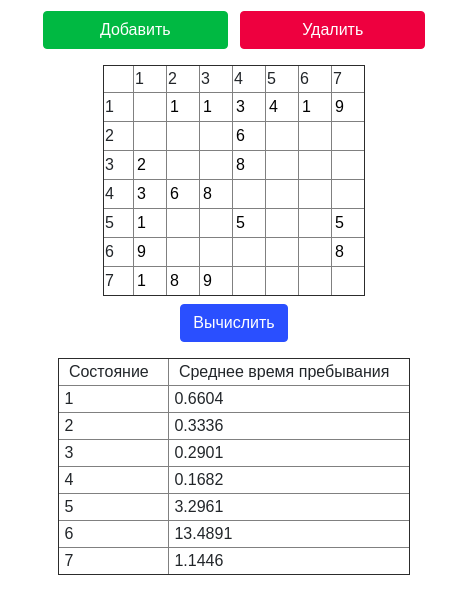
\includegraphics[width=0.6\textwidth]{images/scr02.png}
    \caption{Результат работы для системы из 7 состояний}
    \label{fig:2}
\end{figure}
\begin{figure}[H]
    \centering
    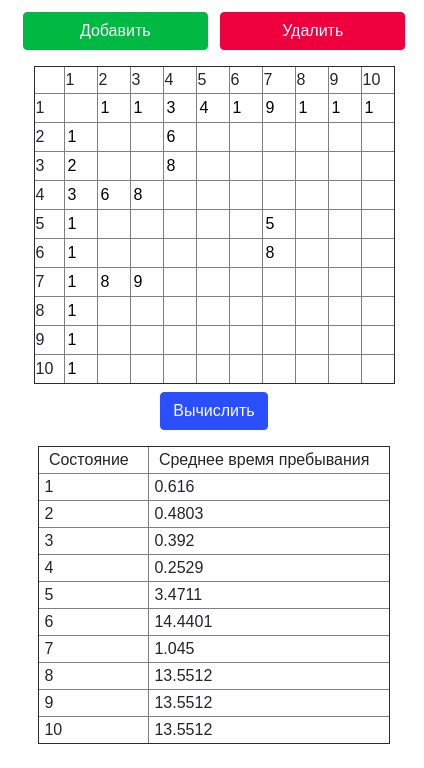
\includegraphics[width=0.6\textwidth]{images/scr03.png}
    \caption{Результат работы для системы из 10 состояний}
    \label{fig:3}
\end{figure}

\chapter*{\hfill{}ВЫВОД\hfill{}}

Была реализована программа, которая для сложной системы S, имеющей не более 10 состояний, рассчитывает среднее время нахождения системы в предельных состояниях, то есть при установившемся режиме работы.
